% --
% wavenets

\section{Experiments on Wavenets}\label{exp_wavenet}
Very few experiments were performed on the Wavenet architecture because of its complex model structure and heavy computational footprint, as already mentioned in \rsec{nn_arch_wavenet}.
The Wavenet model requires a generous amount of time and energy consumption for very few training epochs.
Further the experiments showed poor results on the accuracy of classifying speech commands.
This architecture is therefore left for future research.
Nevertheless, this section presents the best performing Wavenet model on the KWS task.
The training details for this model were 500 examples per each one of the L12 labels, 100 epochs, a learning rate of $0.001$ for 10 epochs and a changing to a learning rate of $0.0001$ and a usual batch size of 32.
\rfig{exp_wavenet_acc} shows the accuracy score for the training and \rfig{exp_wavenet_confusion} provides the confusion matrix on the test set.
However, the best achieved accuracy on the test set was merely \SI{38.83}{\percent}.
\begin{figure}[!ht]
  \centering
  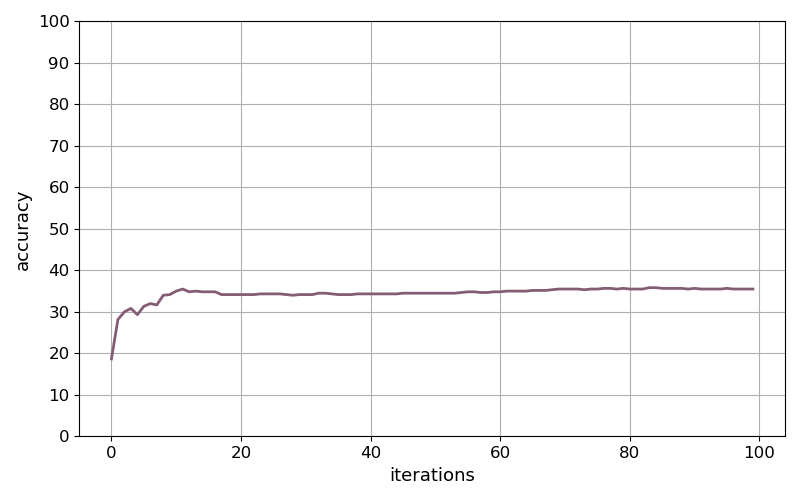
\includegraphics[width=0.45\textwidth]{./5_exp/figs/exp_wavenet_acc.png}
  \caption{Accuracies on the validation set during the training of the Wavenet model with classification extension.}
  \label{fig:exp_wavenet_acc}
\end{figure}
\begin{figure}[!ht]
  \centering
  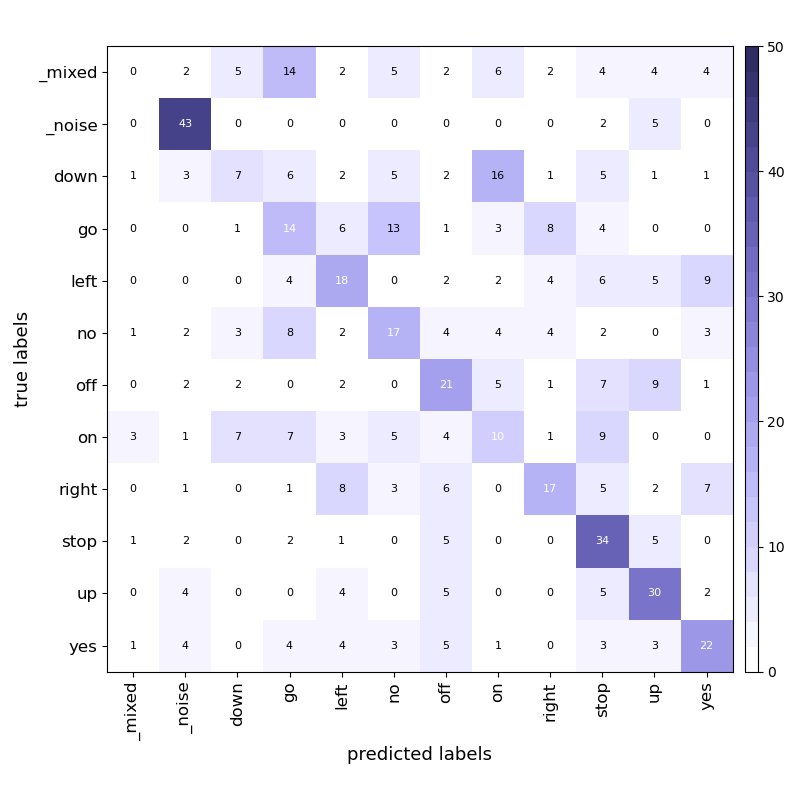
\includegraphics[width=0.45\textwidth]{./5_exp/figs/exp_wavenet_confusion_test.png}
  \caption{Confusion matrix on the test set evaluated on the trained Wavenet model.}
  \label{fig:exp_wavenet_confusion}
\end{figure}
\FloatBarrier
\noindent